

%\subsubsection*{Resultados obtenidos}
%Nota: Al ser los resultados de los experimentos sobre ambos tests muy similares, decidimos analizarlos en conjunto.

\subsubsection*{Tests KNN}

\begin{figure}[H]
\begin{subfigure}[h]{0.62\linewidth}
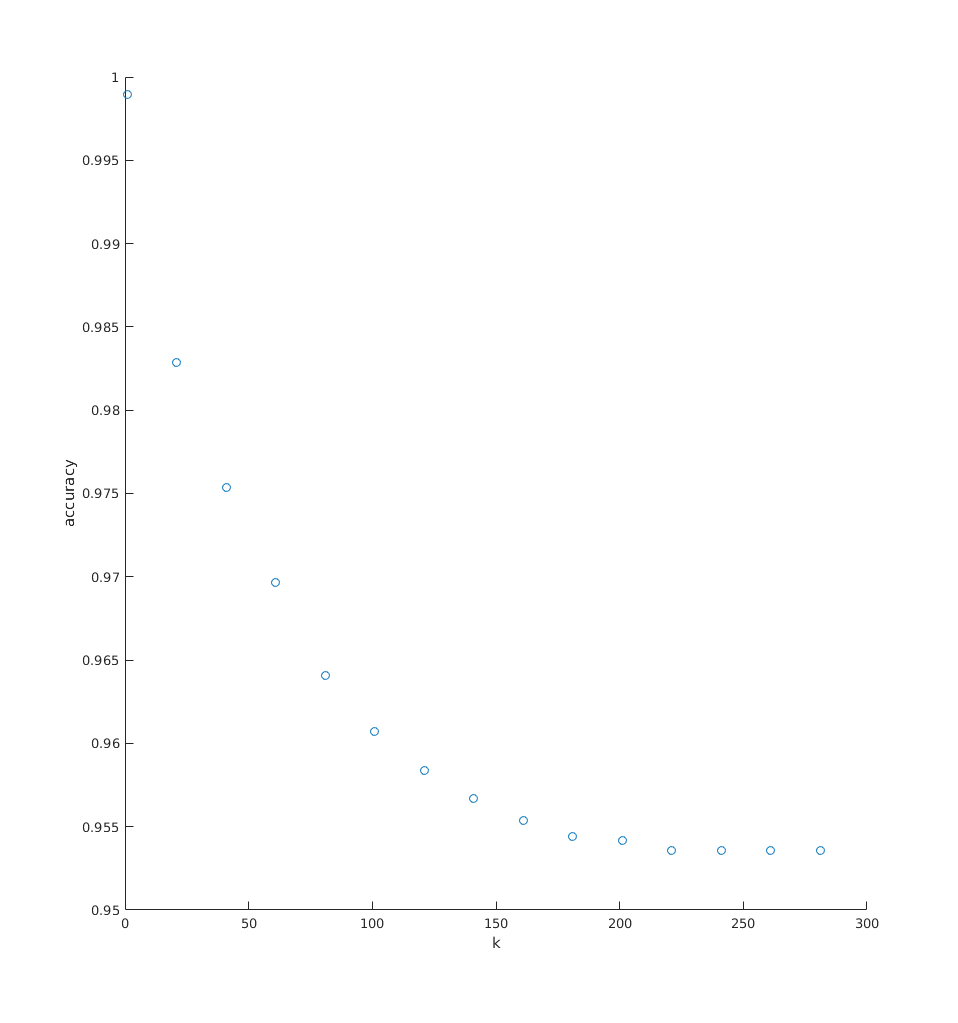
\includegraphics[width=\linewidth]{img/k_knn_accu.png}
\caption{Utilizando imágenes reducidas}
\end{subfigure}
\hfill
\begin{subfigure}[h]{0.62\linewidth}
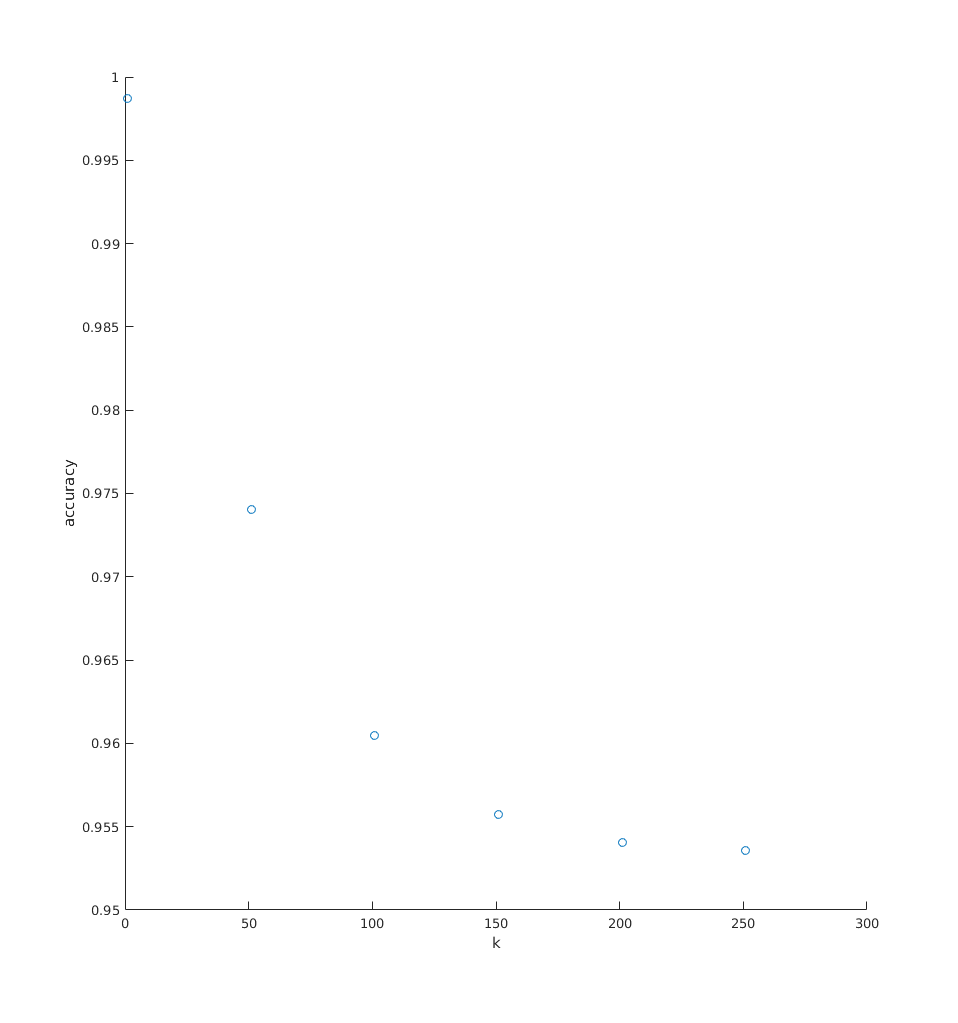
\includegraphics[width=\linewidth]{img/big_k_knn_accu.png}
\caption{Utilizando imágenes grandes}
\end{subfigure}%
\caption{Accuracy vs K con KNN sin PCA}
\end{figure}

En ambos casos obtenemos resultados similares, un Accuracy más grande a menor K, siendo K = 1 el valor óptimo, al menos en este caso.
%Dados los resultados, en este caso consideramos que utilizando un valor de K cercano a 10 obtenemos la mejor relación (dentro de nuestro set de tests).\newline
%Por un lado evitamos el problema que ocurre cuando K es demasiado grande y por otro, tomamos una cantidad de imágenes cercanas suficiente como para minimizar el impacto de algún outsider. Aun que cabe destacar que en este caso particular K = 1 tuvo un mejor comportamiento de lo que esperabamos, consideramos que sería arriesgado tomarlo como valor confiable con otros sets de imágenes.

%%%%%%%%%%%%%%%%%%%%%%%%%%%%%%%%%%%%%%%%%%%%%%%%%%%%%%%%%%%%%%%%%%%%%

\begin{figure}[H]
	\centering
	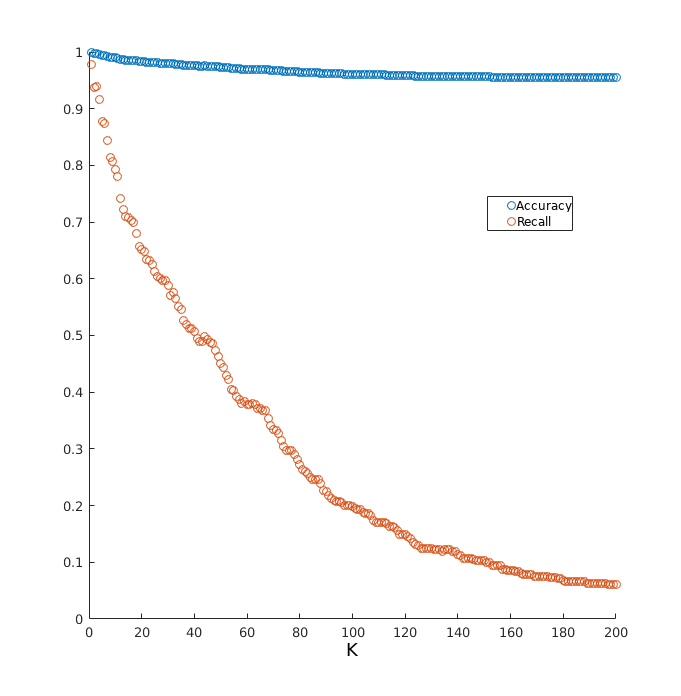
\includegraphics[width=0.8\textwidth]{img/Acc_recall_k_knn.png}
	\caption{Accuracy y Recall vs K (sin PCA)}
	\label{fig: Accuracy y Recall vs K (sin PCA)}
\end{figure}

En este gráfico encontramos algo similar al anterior, si bien se nota un descenso en Accuracy a medida que aumenta K, con el cambio de escala se puede apreciar que el mismo es muy leve.
Por el contrario, sí encontramos que Recall disminuye considerablemente a medida que K crece. En este caso es esta métrica la que nos da más elementos para concluir que K = 1 es la mejor opción.


%%%%%%%%%%%%%%%%%%%%%%%%%%%%%%%%%%%%%%%%%%%%%%%%%%%%%%%%%%%%%%%%%%%%%


%%%%%%%%%%%%%%%%%%%%%%%%%%%%%%%%%%%%%%%%%%%%%%%%%%%%%%%%%%%%%%%%%%%%%
%\begin{figure}[H]
%	\centering	
%	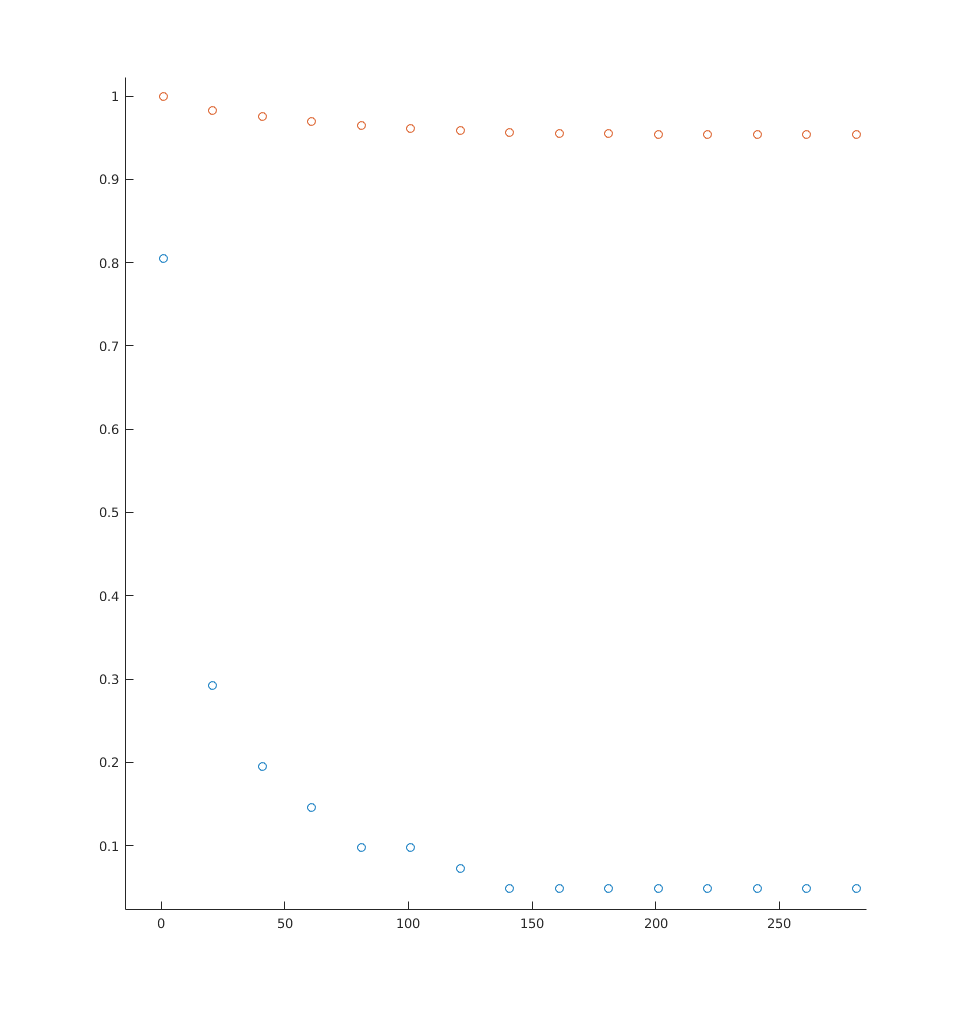
\includegraphics[width=0.8\textwidth]{img/acu_pre.png}
%	\caption{Accuracy y Precision vs K}
%	\label{fig: Accuracy y Precision vs K con KNN}
%\end{figure}

%En este experimento estudiamos cómo es que la cantidad de vecinos cercanos afecta a las métricas Accuracy y Recall.
%
%

%Lo que encontramos no fue muy distinto de lo esperado. En la figura anterior vimos la forma en la que Accuracy variaba en función de la cantidad de vecinos cercanos. Al cambiar la escala, observamos que la variación es bastante leve, pero como explicamos, por ejemplo elegir un K = 250 definitivamente no es una buena elección.
%
%Para tener un sistema robusto necesitamos un valor de (la métrica) recall relativamente alto. Luego en función de lo que nos indica el gráfico nuevamente un valor cercano a K = 1 nos parece adecuado.
%%%%%%%%%%%%%%%%%%%%%%%%%%%%%%%%%%%%%%%%%%%%%%%%%%%%%%%%%%%%%%%%%%%%%
\begin{figure}[H]
\begin{subfigure}[h]{0.62\linewidth}
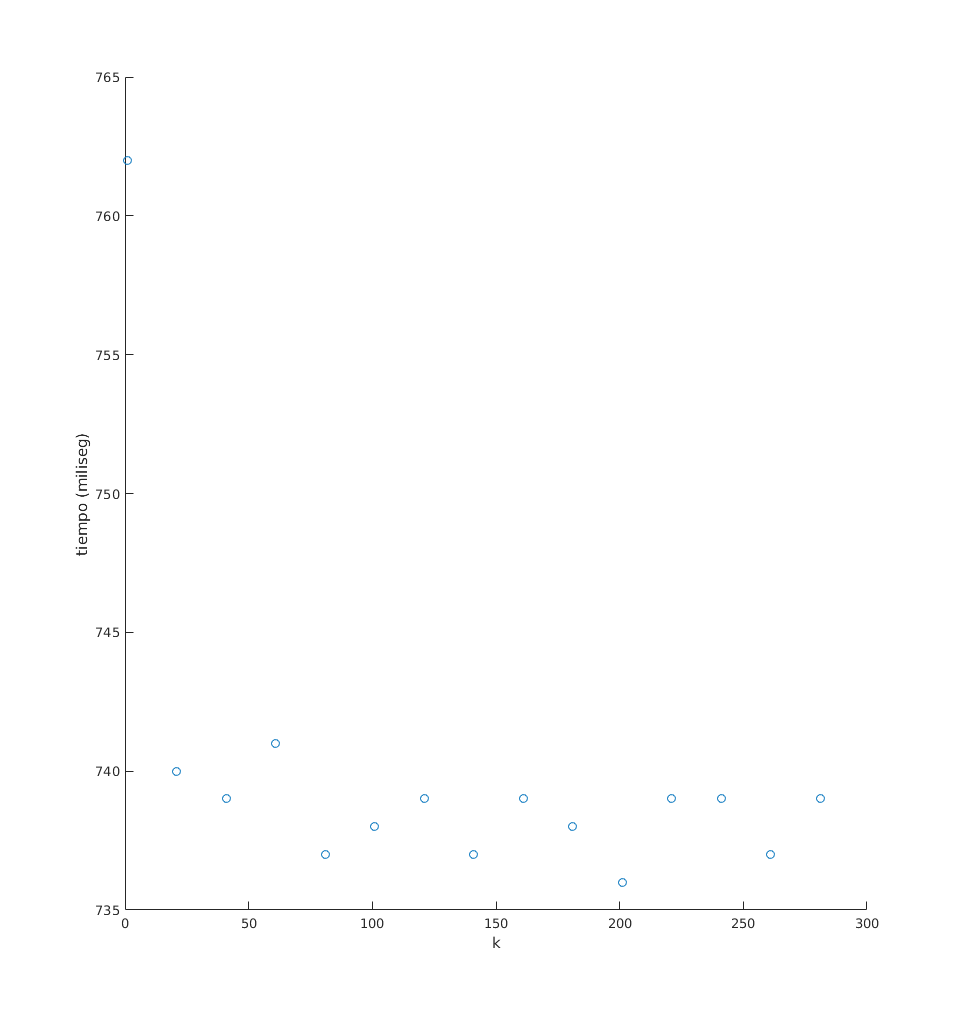
\includegraphics[width=\linewidth]{img/k_knn_tiempo.png}
\caption{Utilizando imágenes reducidas}
\end{subfigure}
\hfill
\begin{subfigure}[h]{0.62\linewidth}
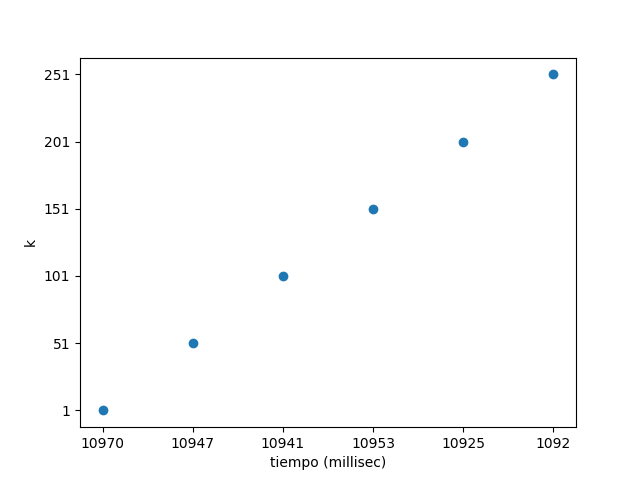
\includegraphics[width=\linewidth]{img/big_k_knn_tiempo.png}
\caption{Utilizando imágenes grandes}
\end{subfigure}%
\caption{Tiempo vs K con KNN sin PCA}
\end{figure}


En este caso no logramos identificar ningún patrón evidente. Si bien en el segundo gráfico se observan algúnas diferencias, en realidad representan pequeñas variaciones en el tiempo de ejecución que no consideramos relevantes.
Esto nos parece razonable, dado que por la forma de nuestra implementación calculamos la distancia con cada una de las imágenes y elegir un K mayor implica muy pocos cálculos adicionales.
%%%%%%%%%%%%%%%%%%%%%%%%%%%%%%%%%%%%%%%%%%%%%%%%%%%%%%%%%%%%%%%%%%%%%


\subsubsection*{Conclusiones del test}
Dados los resultados resulta evidente que cuánto más chico el K mejor se comportan nuestras métricas, luego concluímos que K = 1 es el valor óptimo.
Esto tiene sentido, sin embargo en caso de tener que implementar este problema en la vida real creemos que nos encontraríamos con outliers que pueden afectar el resultado, ya que con un solo vecino cercano tenemos un sistema poco robusto, por lo que elegiríamos un K un poco más grande pero cercano a 1.

%%%%%%%%%%%%%%%%%%%%%%%%%%%%%%%%%%%%%%%%%%%%%%%%%%%%%%%%%%%%%%%%%%%%%
\subsubsection*{Test con KNN + PCA}
Aquí evaluamos cómo se comporta nuestra implementación con PCA, para eso vamos a repetir los tests anteriores pero esta vez utilizando KNN+PCA.
De acuerdo a lo concluído de los tests anteriores inferimos que utilizar K = 1 o algún valor cercano sería lo mejor. 



%%%%%%%%%%%%%%%%%%%%%%%%%%%%%%%%%%%%%%%%%%%%%%%%%%%%%%%%%%%%%%%%%%%%%
\begin{figure}[H]
	\centering
	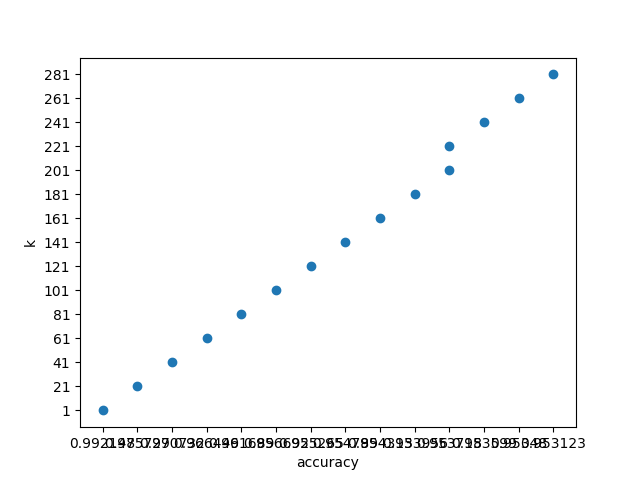
\includegraphics[width=0.8\textwidth]{img/k_pca_accu.png}
	\caption{Accuracy vs K con KNN + PCA}
	\label{fig:K vs Accuracy con KNN + PCA}
\end{figure}

En este caso observamos una estrecha relación entre cuántos vecinos cercanos tomamos y el Accuracy.
Nuevamente K = 1 parece ser el valor óptimo.

%%%%%%%%%%%%%%%%%%%%%%%%%%%%%%%%%%%%%%%%%%%%%%%%%%%%%%%%%%%%%%%%%%%%%

\begin{figure}[H]
\begin{subfigure}[h]{0.62\linewidth}
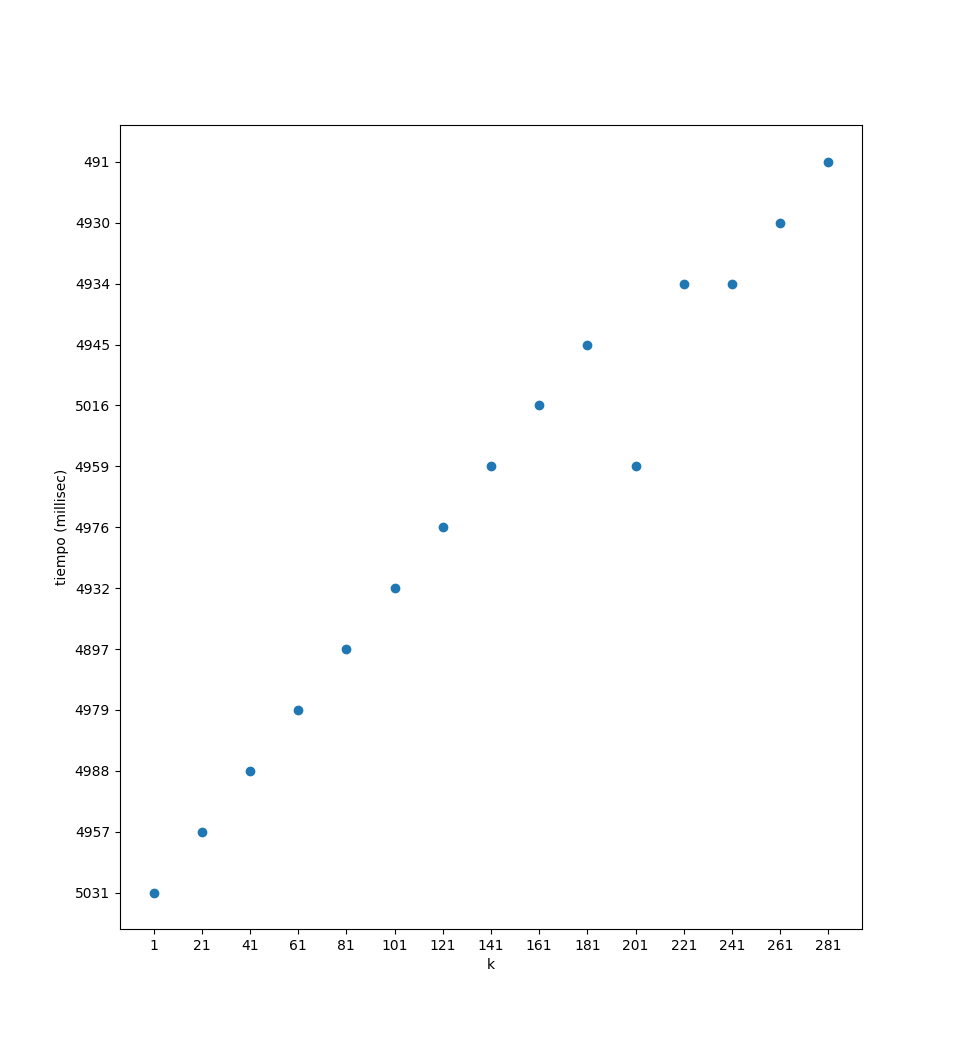
\includegraphics[width=\linewidth]{img/k_pca_tiempo.png}
\caption{Utilizando imágenes reducidas}
\end{subfigure}
\hfill
\begin{subfigure}[h]{0.62\linewidth}
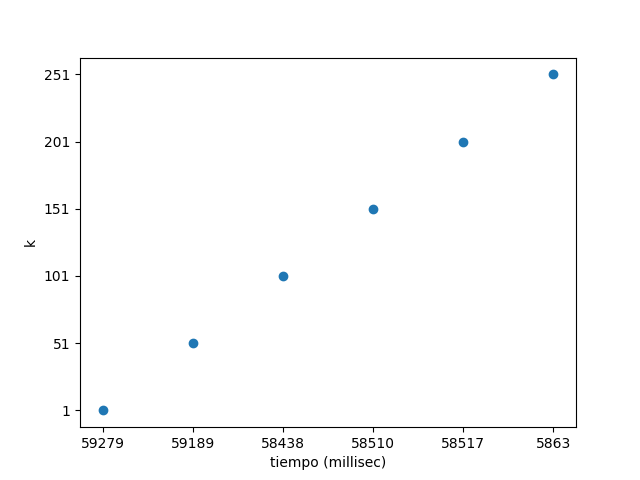
\includegraphics[width=\linewidth]{img/big_k_pca_tiempo.png}
\caption{Utilizando imágenes grandes}
\end{subfigure}%
\caption{Tiempo vs. K con KNN+PCA}
\end{figure}
Este caso es muy similar al visto sin PCA (Figura 3), no notamos diferencias relevantes.

Nótese que al calcular el tiempo incluimos desde el principio hasta el final del algoritmo. Para apreciar mejor la función de PCA tendríamos que haber calculado el tiempo del reconocimiento sin contar el cálculo de PCA. Este fue un hecho que notamos una vez terminada la experimentación pero sería un experimento interesante, que dejaremos para un futuro.\newline
Sin embargo vimos que PCA funciona correctamente en cuanto a nuestras métricas y por nuestra implementación, al trabajar con una matriz más chica obtendríamos una reducción en el tiempo de ejecución (tal como observamos al probar KNN sin PCA con el set de imágenes chico y el grande), con esto podemos deducir que el reconocimiento una vez aplicado PCA tarda menos y a la vez sigue siendo efectivo.

%%%%%%%%%%%%%%%%%%%%%%%%%%%%%%%%%%%%%%%%%%%%%%%%%%%%%%%%%%%%%%%%%%%%%

\begin{figure}[H]
\begin{subfigure}[h]{0.62\linewidth}
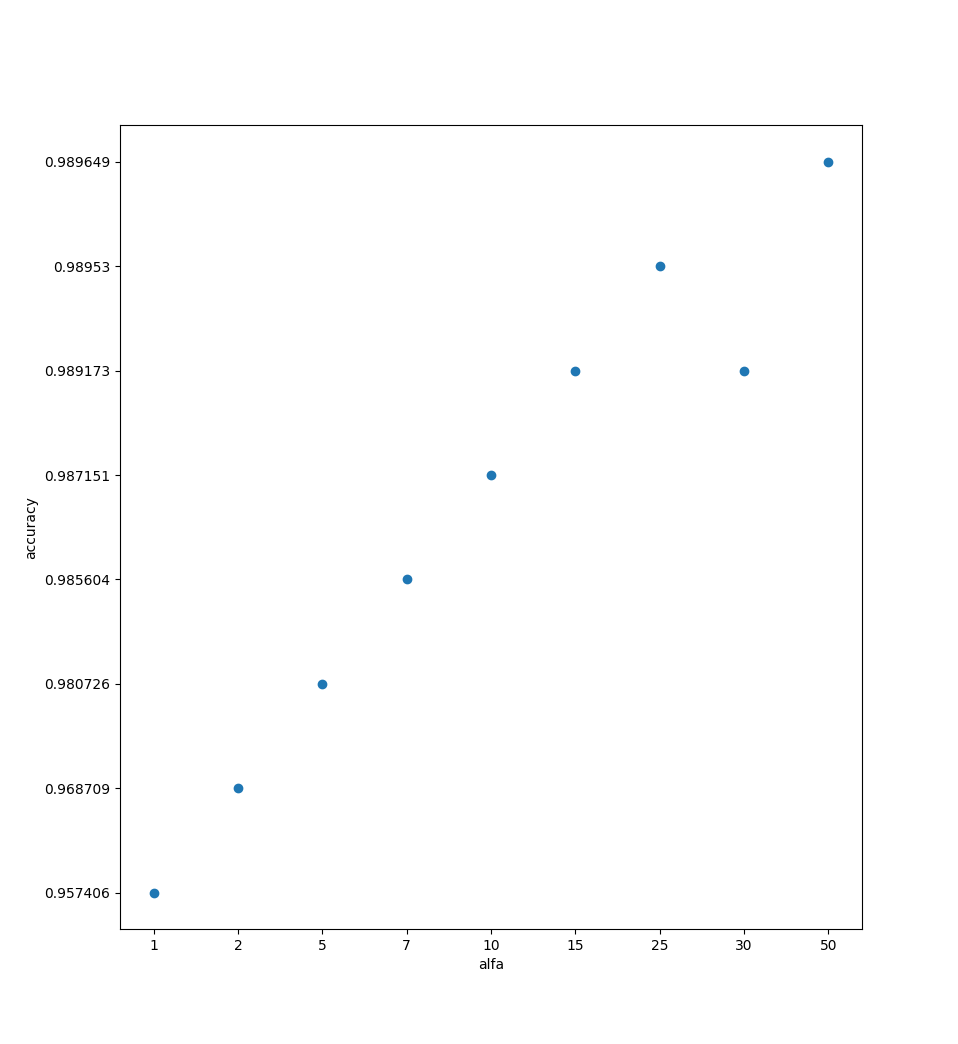
\includegraphics[width=\linewidth]{img/alfa_pca_accu.png}
\caption{Utilizando imágenes reducidas}
\end{subfigure}
\hfill
\begin{subfigure}[h]{0.62\linewidth}
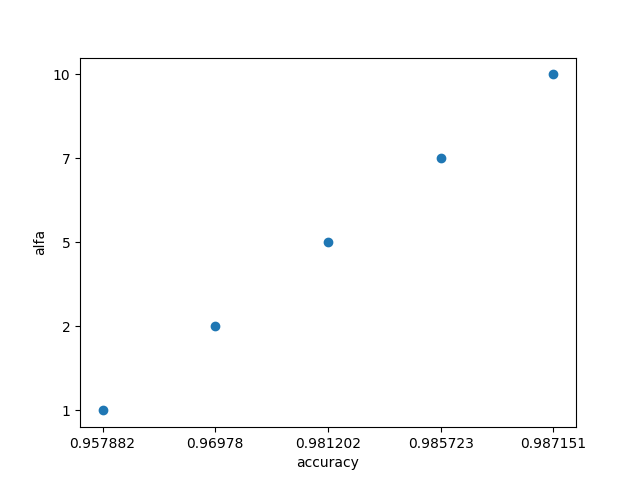
\includegraphics[width=\linewidth]{img/big_alfa_pca_accu.png}
\caption{Utilizando imágenes grandes}
\end{subfigure}%
\caption{Accuracy vs $\alpha$ con KNN+PCA}
\end{figure}

En este caso podemos observar una relación entre las dos variables, a medida que el $\alpha$ aumenta vemos como también lo hace nuestro accuracy.
Como expresamos anteriormente, debido al funcionamiento de PCA esperábamos que a mayor $\alpha$, obtendríamos una mejor reconstrucción y por lo tanto mejores resultados (en todas nuestras métricas en general).

Pero a su vez vimos que un $\alpha$ muy elevado resultaría en un aumento del tiempo de ejecución, no obstante en este gráfico vemos como las diferencias entre accuracy son cada vez menores, es decir como disminuye la pendiente (por ejemplo entre $\alpha$ = 10 y $\alpha$ = 50).

En base a los resultados obtenidos concluimos que un valor de $\alpha$ cercano a 10 nos daría un buen balance entre la cantidad de componentes principales y la efectividad (la cuál disminuye un poco, pero a cambio trabajamos con imágenes mucho más chicas).

Se puede ver en el gráfico a) que el valor máximo probado es $\alpha$ = 50 mientras que en el gráfico b) es $\alpha$ = 10. Esto se debe a que al trabajar en b) con imágenes más grandes requería mucho tiempo de ejecución ya que en los tests se realiza el preprocesamiento de las imágenes en cada corrida, por esto es que probamos solo hasta ese valor, donde igualmente podemos notar la forma del gráfico.

%%%%%%%%%%%%%%%%%%%%%%%%%%%%%%%%%%%%%%%%%%%%%%%%%%%%%%%%%%%%%%%%%%%%%
\begin{figure}[H]
\begin{subfigure}[h]{0.62\linewidth}
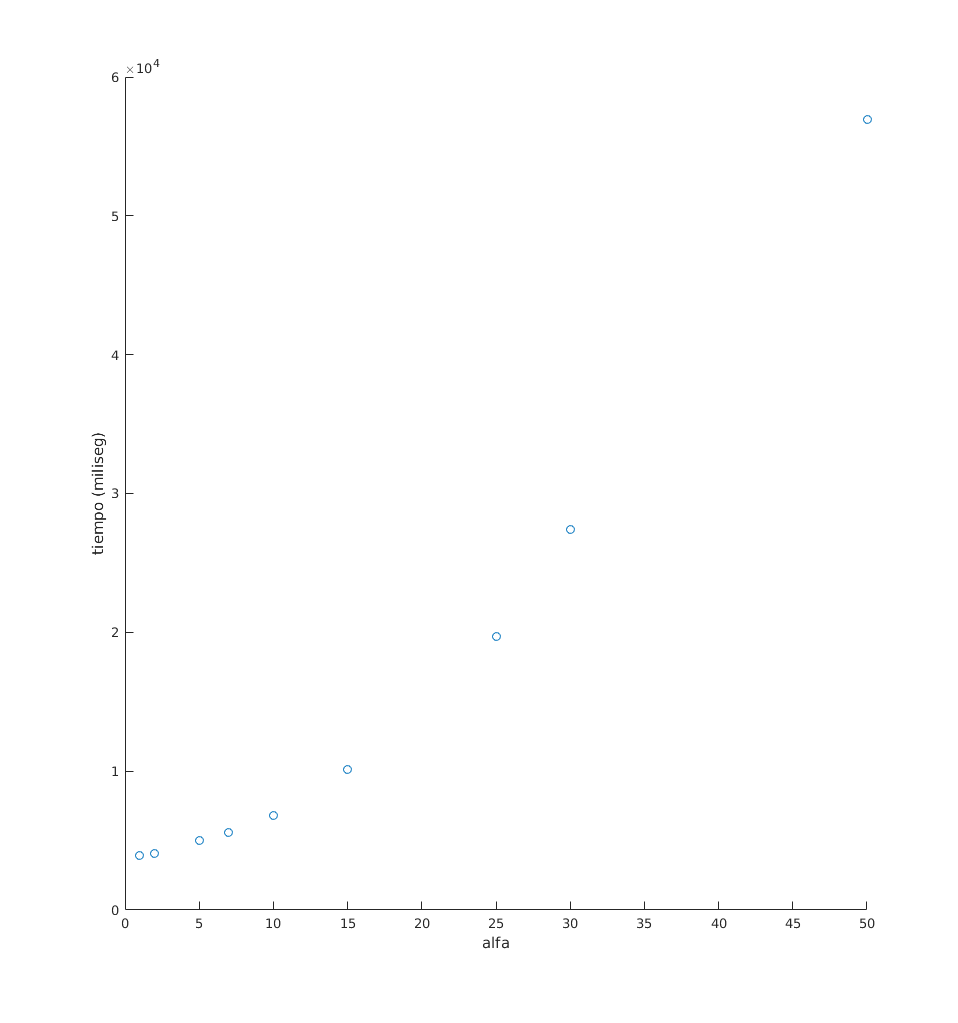
\includegraphics[width=\linewidth]{img/alfa_pca_tiempo.png}
\caption{Utilizando imágenes reducidas}
\end{subfigure}
\hfill
\begin{subfigure}[h]{0.62\linewidth}
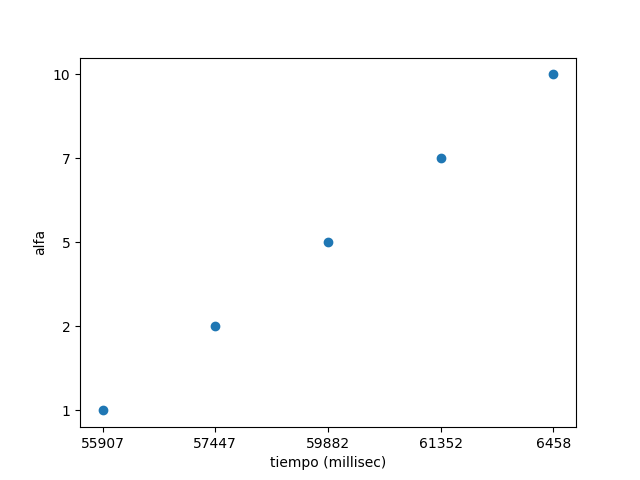
\includegraphics[width=\linewidth]{img/big_alfa_pca_tiempo.png}
\caption{Utilizando imágenes grandes}
\end{subfigure}%
\caption{Tiempo vs $\alpha$ con KNN+PCA}
\end{figure}

Tal como esperábamos vemos que a medida que el $\alpha$ aumenta (es decir, cuantas más componentes principales tengamos), el tiempo de ejecución también lo hace.

Luego, en línea con los resultados de los gráficos anteriores (Accuracy vs $\alpha$) podemos volver a afirmar que un $\alpha$ cercano a 10 sería un buen balance. En a) notamos que si tomáramos $\alpha$ = 30, tardaría aproximadamente el triple y no obtendríamos una mejora en el accuracy que valga la pena.
%%%%%%%%%%%%%%%%%%%%%%%%%%%%%%%%%%%%%%%%%%%%%%%%%%%%%%%%%%%%%%%%%%%%%
\begin{figure}[H]
	\centering
	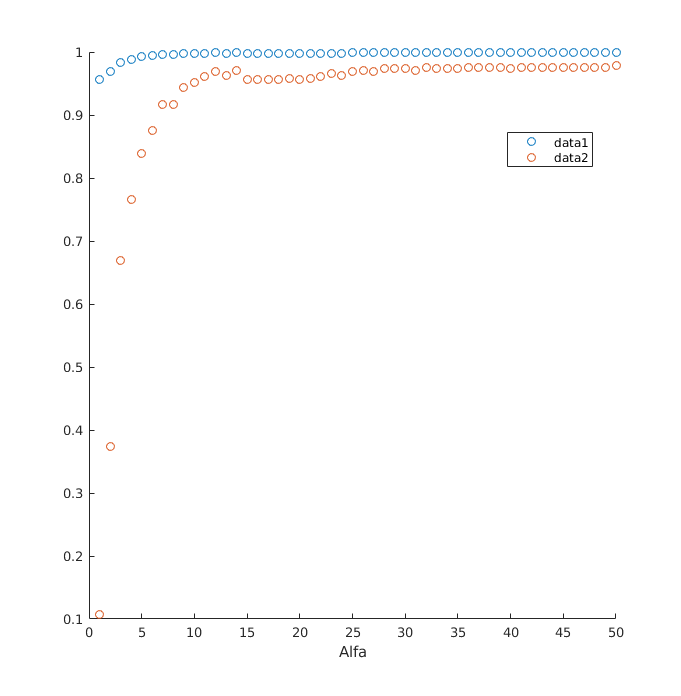
\includegraphics[width=0.8\textwidth]{img/Acc_recall_alfa_pca.png}
	\caption{Accuracy y Recall vs Alfa (con PCA)}
	\label{fig: Accuracy y Recall vs Alfa (con PCA)}
\end{figure}

En este caso al evaluar también recall observamos algo similar, a partir de 10 obtenemos un valor aceptable de esta métrica.
%%%%%%%%%%%%%%%%%%%%%%%%%%%%%%%%%%%%%%%%%%%%%%%%%%%%%%%%%%%%%%%%%%%%%

\begin{figure}[H]
	\centering
	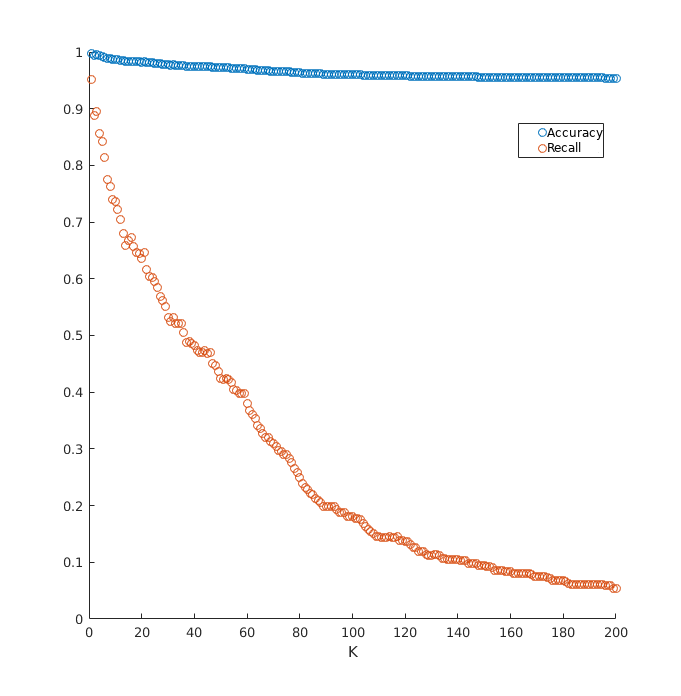
\includegraphics[width=0.8\textwidth]{img/Acc_recall_k_pca.png}
	\caption{Accuracy y Recall vs K (con PCA)}
	\label{fig: Accuracy y Recall vs K (con PCA)}
\end{figure}
Observamos que el resultado es realmente similar al del mismo test llevado a cabo sin PCA, luego por los mismos argumentos utilizados en el caso mencionado decimos que K = 1 es el mejor valor.
También podríamos agregar que el hecho de obtener resultados muy similares al test sin PCA habla bien del funcionamiento de PCA (con $\alpha$ = 10) que obtiene una buena tasa de reconocimiento con muy pocas componentes (lo que equivale a un gran ahorro de espacio).
%%%%%%%%%%%%%%%%%%%%%%%%%%%%%%%%%%%%%%%%%%%%%%%%%%%%%%%%%%%%%%%%%%%%%

Llegamos a la conclusión de que utilizando un valor de K mayor pero cercano a 1 obtenemos la mejor relación (dentro de nuestro set de tests).
Por un lado evitamos el problema que ocurre cuando K es demasiado grande y por otro, tomamos una cantidad de imágenes cercanas suficiente como para minimizar el impacto de algún outsider.


